% Budget Control and Monitoring Process
% TikZ diagram for Chapter 2

\documentclass[tikz,border=10pt]{standalone}
\usepackage{tikz}
\usetikzlibrary{shapes,arrows,positioning,fit,backgrounds}

\begin{document}

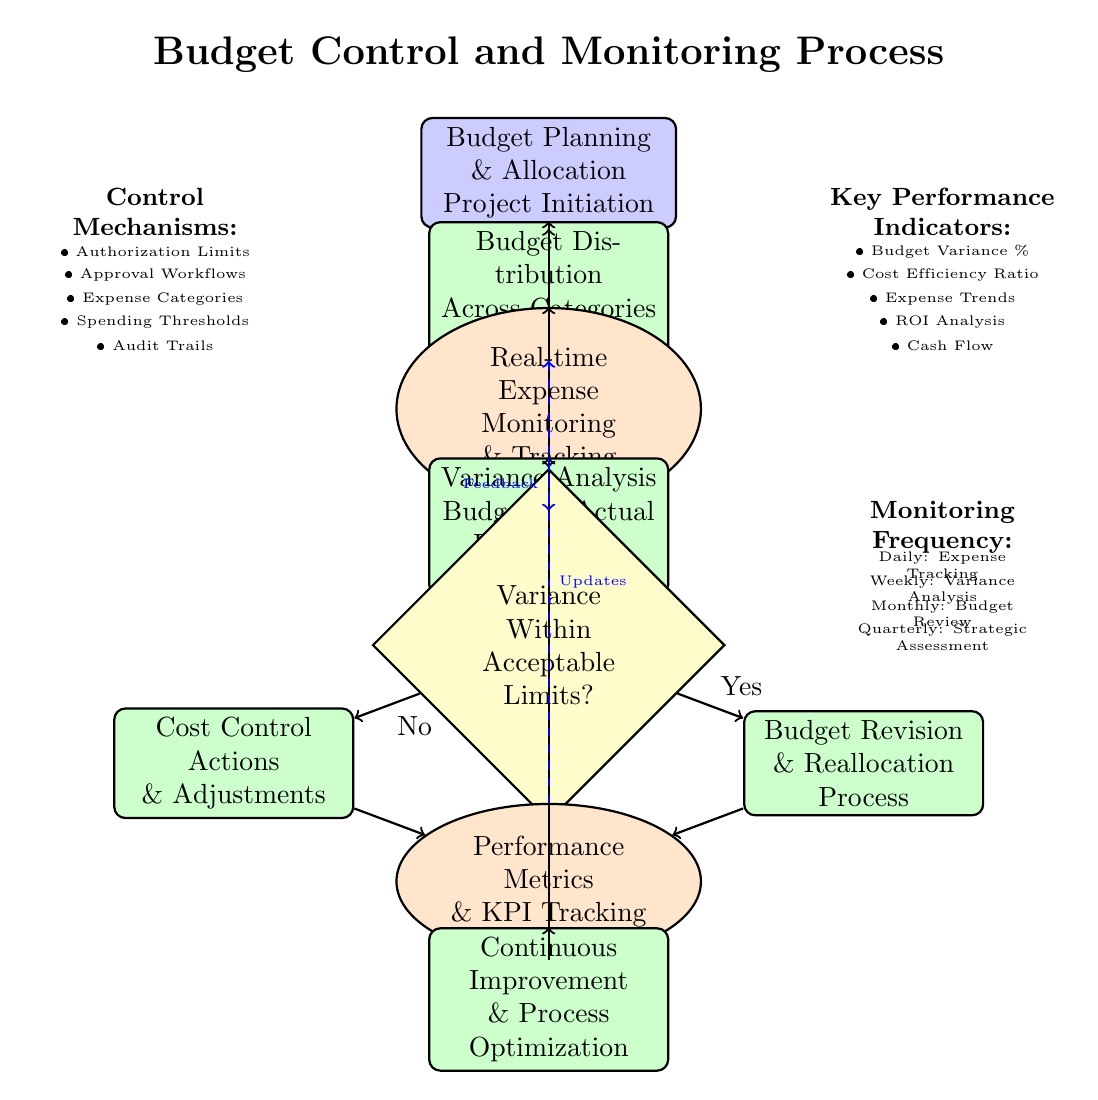
\begin{tikzpicture}[
    node distance=1.5cm,
    auto,
    thick,
    main node/.style={rectangle, draw, fill=blue!20, text width=3cm, text centered, rounded corners, minimum height=1cm},
    decision node/.style={diamond, draw, fill=yellow!20, text width=2.5cm, text centered, minimum height=1cm},
    process node/.style={rectangle, draw, fill=green!20, text width=2.8cm, text centered, rounded corners, minimum height=0.8cm},
    monitor node/.style={ellipse, draw, fill=orange!20, text width=2.5cm, text centered, minimum height=0.8cm}
]

% Title
\node[text width=12cm, text centered, font=\Large\bfseries] (title) at (0,8) {Budget Control and Monitoring Process};

% Budget Planning
\node[main node] (budget_planning) at (0,6.5) {Budget Planning\\\& Allocation\\Project Initiation};

% Budget Distribution
\node[process node] (budget_distribution) at (0,5) {Budget Distribution\\Across Categories\\\& Activities};

% Expense Monitoring
\node[monitor node] (expense_monitoring) at (0,3.5) {Real-time Expense\\Monitoring\\\& Tracking};

% Variance Analysis
\node[process node] (variance_analysis) at (0,2) {Variance Analysis\\Budget vs Actual\\Performance Review};

% Variance Decision
\node[decision node] (variance_decision) at (0,0.5) {Variance\\Within\\Acceptable Limits?};

% Cost Control Actions
\node[process node] (cost_control) at (-4,-1) {Cost Control\\Actions\\\& Adjustments};

% Budget Revision
\node[process node] (budget_revision) at (4,-1) {Budget Revision\\\& Reallocation\\Process};

% Performance Metrics
\node[monitor node] (performance_metrics) at (0,-2.5) {Performance Metrics\\\& KPI Tracking};

% Continuous Improvement
\node[process node] (improvement) at (0,-4) {Continuous Improvement\\\& Process Optimization};

% Arrows
\draw[->] (budget_planning) -- (budget_distribution);
\draw[->] (budget_distribution) -- (expense_monitoring);
\draw[->] (expense_monitoring) -- (variance_analysis);
\draw[->] (variance_analysis) -- (variance_decision);
\draw[->] (variance_decision) -- node {No} (cost_control);
\draw[->] (variance_decision) -- node {Yes} (budget_revision);
\draw[->] (cost_control) -- (performance_metrics);
\draw[->] (budget_revision) -- (performance_metrics);
\draw[->] (performance_metrics) -- (improvement);
\draw[->] (improvement) -- (budget_planning);

% Feedback loops
\draw[->, dashed, blue] (variance_analysis) -- node[left, font=\tiny] {Feedback} (expense_monitoring);
\draw[->, dashed, blue] (performance_metrics) -- node[right, font=\tiny] {Updates} (budget_distribution);

% Key Performance Indicators
\node[text width=3cm, text centered, font=\small\bfseries] (kpi_title) at (5,6) {Key Performance\\Indicators:};
\node[text width=3cm, text centered, font=\tiny] (kpi1) at (5,5.5) {• Budget Variance \%};
\node[text width=3cm, text centered, font=\tiny] (kpi2) at (5,5.2) {• Cost Efficiency Ratio};
\node[text width=3cm, text centered, font=\tiny] (kpi3) at (5,4.9) {• Expense Trends};
\node[text width=3cm, text centered, font=\tiny] (kpi4) at (5,4.6) {• ROI Analysis};
\node[text width=3cm, text centered, font=\tiny] (kpi5) at (5,4.3) {• Cash Flow};

% Control Mechanisms
\node[text width=3cm, text centered, font=\small\bfseries] (control_title) at (-5,6) {Control Mechanisms:};
\node[text width=3cm, text centered, font=\tiny] (control1) at (-5,5.5) {• Authorization Limits};
\node[text width=3cm, text centered, font=\tiny] (control2) at (-5,5.2) {• Approval Workflows};
\node[text width=3cm, text centered, font=\tiny] (control3) at (-5,4.9) {• Expense Categories};
\node[text width=3cm, text centered, font=\tiny] (control4) at (-5,4.6) {• Spending Thresholds};
\node[text width=3cm, text centered, font=\tiny] (control5) at (-5,4.3) {• Audit Trails};

% Timeline
\node[text width=3cm, text centered, font=\small\bfseries] (timeline_title) at (5,2) {Monitoring\\Frequency:};
\node[text width=3cm, text centered, font=\tiny] (timeline1) at (5,1.5) {Daily: Expense\\Tracking};
\node[text width=3cm, text centered, font=\tiny] (timeline2) at (5,1.2) {Weekly: Variance\\Analysis};
\node[text width=3cm, text centered, font=\tiny] (timeline3) at (5,0.9) {Monthly: Budget\\Review};
\node[text width=3cm, text centered, font=\tiny] (timeline4) at (5,0.6) {Quarterly: Strategic\\Assessment};

\end{tikzpicture}

\end{document}
